\subsection{Design og Implementering}

Da \gls{SL} skulle designes blev det i første iteration klart at der ville opstå et væld af klasser i dette bibliotek. Det blev derfor besluttet at disse skulle være tilgængelige via en .dll fil som alle systemer fik adgang til og disse klasser blev efter grundige overvejelser indkapslet i de pakker som ses på figur \ref{fig:oversigtSL}. Pakkerne blev herefter udviklet efter nødvendighed igennem de forskellige iterationer, Hvilket satte SOLID designprincipperne på noget af en prøve.

\begin{figure}[!h]
    \centering
    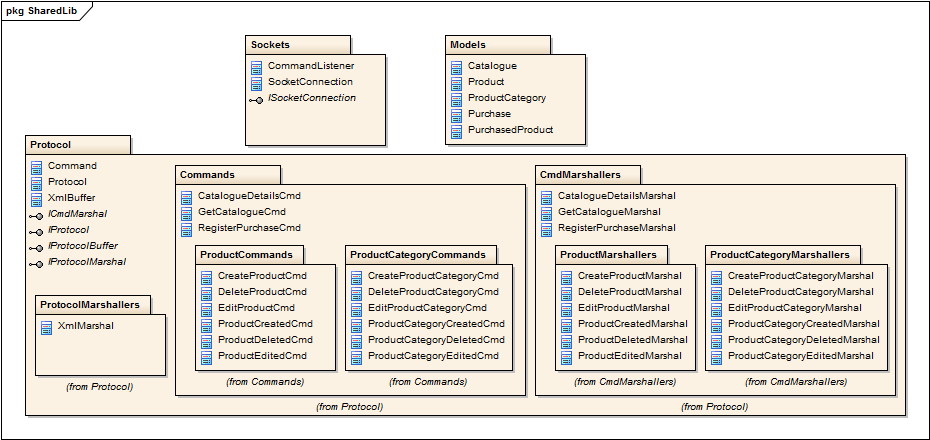
\includegraphics[width=1.0\textwidth]{Systemdesign/SharedLib/Images/SharedLib_Package2.png}
    \caption{Oversigt over alle pakker i SharedLib}
    \label{fig:oversigtSL}
\end{figure}

Herunder ses en kort beskrivelse af de forskellige pakker, og hvad de indeholder.

\begin{itemize}
\item \textbf{Models} indeholder datamodeller der i de forskellige systemer bruges som skabeloner. 
\item \textbf{Sockets} indeholder klasser til asynkron forbindelse til \gls{CS} samt de events der bliver raised a \gls{CS}.
\item \textbf{Protocol} indeholder hele protokollen og er denne der bruges til kommunikation mellem alle delsystemer.
\item \textbf{ProtocolMarshallers} indeholder de kodesprog der kan kommunikeres med.
\item \textbf{Commands} indeholder de forskellige kommandoer der bruges til at sende information over protokollen.
\item \textbf{ProductCommands} indeholder kommandoer der er specifikke for produkter.
\item \textbf{ProductCategoryCommands} indeholder kommandoer der er specifikke for produktkategorier.
\item \textbf{CmdMarshallers} indeholder marshallers som har til opgave at parse de forskellige kommandoer til og fra XML.
\item \textbf{ProductMarshallers} indeholder marshallers der er specifikke for produkter.
\item \textbf{ProductCategoryMarshallers} indeholder marshallers der er specifikke for produktkategorier.
\end{itemize}

\textbf{Funktionalitet}\\

\gls{SL}'s hovedformål var fra starten at sørge for at udviklerne på de forskellige delsystemer ikke skulle tænke over at parse deres data til XML og tilbage til brugbar data. Derfor blev det besluttet at ligge alt denne funktionalitet et sted. Denne funktionalitet blev siden udvidet til datamodeller hvis nødvendighed opstod da alle delsystemer på denne måde kunne håndtere informationer om f.eks. produkter, på samme måde.\\

Protokollen for \gls{SL} fungerer ved at et givet delsystem f.eks. laver et produkt objekt de gerne vil sende til \gls{CS}, dette pakkes herefter ind i et kommando objekt, Som derefter bliver sendt med som parameter i protokol objektets encode funktion. denne sørger for at produktinformationerne inde i kommando objektet bliver parset til XML og at dette bliver gemt i en string som bliver sendt via socket objektet. For yderligere informationer omkring protokollen, se da afsnit\ref{PROTOKOL}\\


\textbf{Design}\\

Da Design arbejdet af protokollen langsomt begyndte at tage form, kom udfordringen med hvordan der kunne udarbejdes en sekvens af handlinger som så enkelt som muligt kunne tilføje funktionalitet til systemet, men som samtidigt ikke ville sætte det ud af spil eller kræve store revideringer, i og med protokollen var sådan en central del af systemet. Blikket blev hurtigt kastet mod SOLID design principperne da disse kunne gøre netop dette for systemet.

Det første punkt var S, Single responsibility, og her blev udarbejdet ideen om det der senere skulle blive commands og marshallers, det at hver commando skulle have sin egen klasse og sin egen parser og at disse kun skulle have det ene ansvar, netop at videre bringe information og at parse denne.

Næste punkt O, Open-Closed princippet, der ligger op til at systemet skal være åben for tilføjelser men lukket for ændringer, blev også overholdt ved teorien omkring commands og marshallers, da der pludseligt kunne opstå et behov for ny funktionalitet, og at man her ved hjælp af et interface kunne lave en ny implementering og hermed en ny kommando uden af ændre det eksiterende.

\textbf{L'et i SOLID er Liskov's substitutions princip og dette siger at du skal kunne bytte rundt på en subklasse og den klasse denne arver fra, uden at programmet bemærker dette. Dette er i \gls{SL} også tilfældet. Det eneste sted der reelt er arv er fra Command klassen og til de forskellige kommandoer og dette vil ikke give problemer og der brydes derfor ikke med dette princip. UNDERSØG OM DET ER ET PROBLEM MED EKSTRA ATTRIBUTTER???}

I'et var Interface Segregation og betød at hvis der ønskes en specifik funktion i et større system, som bør der så vidt muligt være interfaces der sørger for at den ønskede funktionalitet kan tilgås uden at være tvunget til at tage stilling til og håndtere unødvendige funktioner. Dette opnådede protokollen også da der blev indført interfaces for alle klasser på når Commands som derimod blev en abstrakt klasse der blev nedarvet fra.

D'et og det sidste punkt i SOLID er Dependency inversion og kræver at afhængigheder skal komme nede fra og op. Ment som at en superklasse ikke skal kende til klasser i lavere lag på trods af at den måske bruger dem aktivt, dette skal fungerer via et interface i samme lag, som så bliver implementeret af en klasse i et lavere lag der her udfører disse handlinger. Dette fik protokollen også indført med de mange interfaces der her kunne sørge for at alt afhængighed kom nedefra. Protocol klassen kender f.eks. ikke den XmlMarshaller der finder den korrekte marshaller at bruge, den har et IProtocolMarshaller interface som XmlMarshaller implementere. Det samme for XmlMarshaller der ikke kender til de enkelte marshallers men derimod arbejder med ICmdMarshaller som de forskellige marshallers så har implementeret.\\

Herunder på figur \ref{fig:overklasseSL} ses et overordnet klassediagram for protokollen i \gls{SL} som designet endte ud, og hvor det tydeligt ses hvordan de forskellige interfaces muliggøre kommunikation på tværs af lag.


\begin{figure}[H]
	\centering
	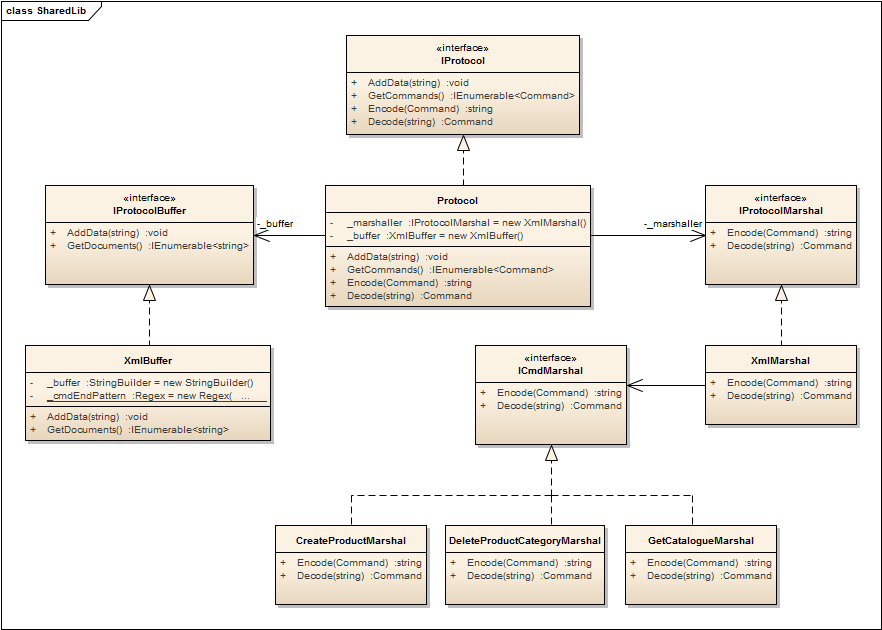
\includegraphics[width=1.0\textwidth]{Systemdesign/SharedLib/Images/SharedLib_Overordnet.png}
	\caption{Klassediagram over \gls{SL}'s protokol}
	\label{fig:overklasseSL}
\end{figure}


\subsection{Models}
Moddellerne i \gls{SL} har fungeret som domæneklasser og har grundlæggende været brugt til at ensrette data på tværs af delsystemerne.

\subsubsection{Klassebeskrivelser}
Herunder ses de forskellige modelklasser i \gls{SL} og der vil til hver klasse være en uddybende forklaring om dennes funktionalitet og ansvar\\

\textbf{Catalogue}\\
Denne klasse indeholder en liste af produktkategorier, der hver især selv indeholder en liste af produkter, se afsnit \ref{PRODUCTCATEGORY} om ProductCategory for yderligere info om disse. Catalogue er det katalog af produkter systemet indeholder og ved boot af et delsystem vil dette som regel kalde en GetCatalogueDetails kommando, som vil give dem en instans af Catalogue med alle produkter i deres enkelte produktkategorier i systemet.

\begin{figure}[H]
    \centering
    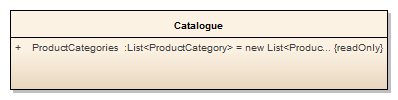
\includegraphics[width=0.6\textwidth]{Systemdesign/SharedLib/Images/Klasser/Model/Catalogue.png}
    \caption{Catalogue}
    \label{fig:klasseModelCata}
\end{figure}

\textbf{Product}\\
Denne klasse er meget brugt igennem hele systemet, den blev tidligt i udviklingen fastlagt så systemerne kunne udvides omkring dette koncept. Product indeholder alle data som for systemet er relevant omkring et produkt.

\begin{figure}[H]
    \centering
    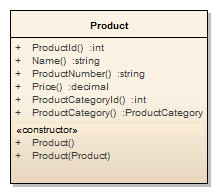
\includegraphics[width=0.4\textwidth]{Systemdesign/SharedLib/Images/Klasser/Model/Product.png}
    \caption{Product}
    \label{fig:klasseModelPrd}
\end{figure}


\textbf{ProductCategory}\label{PRODUCTCATEGORY}\\
Klassen ProductCategory kom ind i en senere iteration og gav muligheden for at placere produkter under samme kategori, f.eks. æble og pære under en kategori der hed "frugt".
ProductCategory har derfor som sagt et navn og derudover også en liste af produkter. 

\begin{figure}[H]
    \centering
    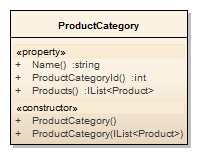
\includegraphics[width=0.4\textwidth]{Systemdesign/SharedLib/Images/Klasser/Model/ProductCategory.png}
    \caption{ProductCategory}
    \label{fig:klasseModelPrdCtg}
\end{figure}


\textbf{PurchasedProduct}\\
Klassen PurchasedProduct blev oprettet da der skulle implementeres funktionalitet omkring salg. Dette nødvendigjorde at der skulle et tidsstempel på produktet der var solgt og at der derudover skulle et antal (hvis flere af samme produkt var købt), prisen på daværende tidspunkt, da den nuværende pris på produktet godt kunne være ændret senere i databasen og til sidst en total pris, som bliver gjort op af antallet og stykprisen. Der blev derudover tilføjet et event til PurchasedProduct da denne også bliver brugt i \gls{KA}'s shoppinglist. Denne skulle vide hvornår antallet i en instans ændres, så grænsefladen kan ændre værdien på skærmen.

\begin{figure}[H]
    \centering
    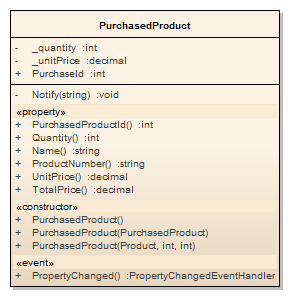
\includegraphics[width=0.6\textwidth]{Systemdesign/SharedLib/Images/Klasser/Model/PurchasedProduct.png}
    \caption{PurchasedProduct}
    \label{fig:klasseModelPurPrd}
\end{figure}


\textbf{Purchase}\\
Denne klasse sørger for at registrere køb fra \gls{KA}. Purchase klassen skal altså simulere et samlet køb af en eller flere varer og bliver derfor også brugt til at danne kvitteringer. Dette betyder altså at klassen har en liste af PurchasedProducts og et tidsstempel for købet.

\begin{figure}[H]
    \centering
    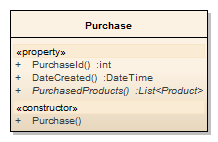
\includegraphics[width=0.4\textwidth]{Systemdesign/SharedLib/Images/Klasser/Model/Purchase.png}
    \caption{Purchase}
    \label{fig:klasseModelPurch}
\end{figure}





\subsection{Protocol}\label{PROTOKOL}
Protokollen til systemet blev tidligt besluttet at skulle fungere ved at sende strenge af XML over en socket forbindelse. Da det kom til den reelle udvikling af hvordan denne XML string skulle genereres blev der opsat nogle begreber til videre udarbejdelse:

\begin{itemize}
\item \textbf{Encode} Der skulle kunne gives et forudbestemt data objekt til en encode funktion der herefter skulle sørge for at generere en passende XML string. 
\item \textbf{Decode} Der skulle ligeledes kunne gives en string med XML som en decode funktion herefter kunne danne et passende data objekt udfra. 
\item \textbf{Commands} De kommandoer der skulle videregives informationer om skulle fungere som objekter der på bagrund af informationen i dem, kunne handles på andetsteds.
\item \textbf{Marshallers} Der skulle ligge noget logik "bagved" protocol objektet, som her skulle sørge for den reelle ændring fra det XML til Data og omvendt. Det blev derfor nødvendigt at lave en Marshaller for hver Command som protocol objektet kunne kalde på.
\end{itemize}

\begin{figure}[H]
    \centering
    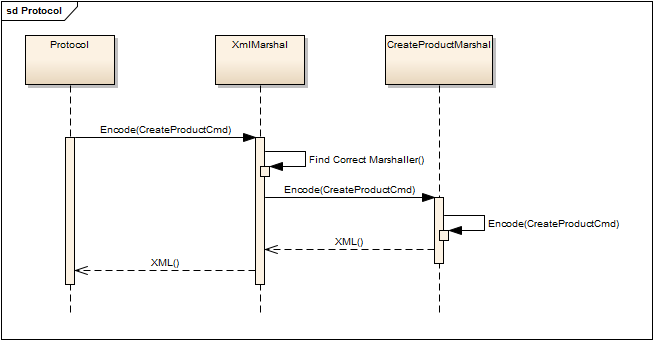
\includegraphics[width=1.0\textwidth]{Systemdesign/SharedLib/Images/Protokol/Protocol_Sek.png}
    \caption{Sekvensdiagram over protokollens encode funktion}
    \label{fig:protocolSek}
\end{figure}

På figur \ref{fig:protocolSek} er der illustreret et scenarie hvor Der bliver kaldt encode med en CreateProduct kommando på protocol objektet, dette kan f.eks. være \gls{AS} der vil oprette et produkt i databasen og derfor skal sende denne besked over socket forbindelsen.

\gls{AS} vil derfor lave en instans af den givne kommando klasse, en instans af protocol klassen. Herefter kaldes Encode fra protocol objektet med kommandoen og denne vil herefter kalde encode med kommandoen på den korrekte marshaller, som til sidst reelt parser objektet om til en XML string og sender dette tilbage gennem XMLMarshal klassen og tilbage til protocol objektet. 

Som det ses på figur \ref{fig:protocolSek}, er der ikke mange kald der bliver lavet når en kommando bliver encoded, Dog sker der en masse logik i de enkelte klasser. Da protocol klassen blev udarbejdet blev det besluttet at der skulle være mulighed for udvidelse af systemet så der kunne sendes med andre kodesprog end XML over socket forbindelserne. derfor blev der oprette et interface til XmlMarshal klassen som denne implementere og dette er derfor det første protocol tager stilling til.

Derefter er der et hav af commands og marshallers, og for at følge Open-Closed princippet skulle det på sigt være muligt at kunne sende andre commandoer over systemet. Derfor tager XmlMarshal stilling til, på baggrund af den indkomne kommandos navn, hvilken Marshaller der er passende for denne kommando og kalder, hvis denne eksistere, encode/decode på denne marshaller.
\subsection{XmlBuffer}
XmlBuffer har til ansvar at tage imod en strøm af data fra en socketforbindelse og opdele XML-dokumenter. Den fungerer ved, at når en klient har modtaget data fra en socket tilføjes dette data til bufferen via AddData(). Herefter kaldes GetDocuments(), som returnerer en liste over de komplette XML-dokumenter, bufferen indeholder. De returnerede dokumenter fjernes derefter fra bufferen.\\

Der blev derudover oprettet et interface, IProtocolBuffer, dette var i tilfælde af at systemet senere skulle udvides med flere buffere, så systemet ville kunne kommunikere med flere/andre dataformater.

\begin{figure}[H]
	\centering
	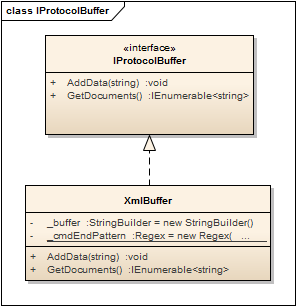
\includegraphics[width=0.4\textwidth]{Systemdesign/SharedLib/Images/Klasser/IProtocolBuffer.png}
	\caption{XmlBuffer der implementerer IProtocolBuffer}
	\label{fig:klasseXmlBuf}
\end{figure}

\subsection{Commands}\label{COMMAND}
Fælles for alle systemerne i dette projekt er at de kommunikerer ved hjælp af kommandoer. 

Der skelnes imellem tre typer af kommandoer:

\begin{itemize}
\item \textbf{Generelle kommandoer} 
\item \textbf{Produkt kommandoer} 
\item \textbf{Produktkategori kommandoer}
\end{itemize}

\textbf{Generelle kommandoer} er kommandoer der ikke er specifikke for hverken Product eller ProductCategory klasserne, og dækker mere overfladiske behov som f.eks. "send mig kataloget med produkter" (GetCatalogueCmd).

På figur \ref{fig:overklasseGen} ses en oversigt over de forskellige generelle kommando klasser der nedarver fra Command klassen.

\begin{figure}[H]
    \centering
    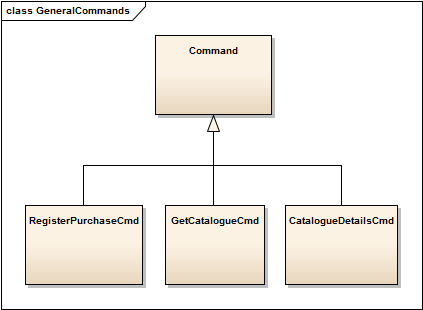
\includegraphics[width=0.6\textwidth]{Systemdesign/SharedLib/Images/Commands/GeneralCommands.png}
    \caption{Oversigt over generelle kommandoer der nedarver fra Command klassen}
    \label{fig:overklasseGen}
\end{figure}

\textbf{Produkt kommandoer} er kommando klasser der er specifikke for Product klassen og medfører ændringer i et givet produkt. Et eksempel på dette kunne være CreateProductCmd, som beder om et produkt skal oprettes i databasen.

På figur \ref{fig:overklassePrd} ses en oversigt over de forskellige produkt kommandoer der nedarver fra Command klassen.

\begin{figure}[H]
    \centering
    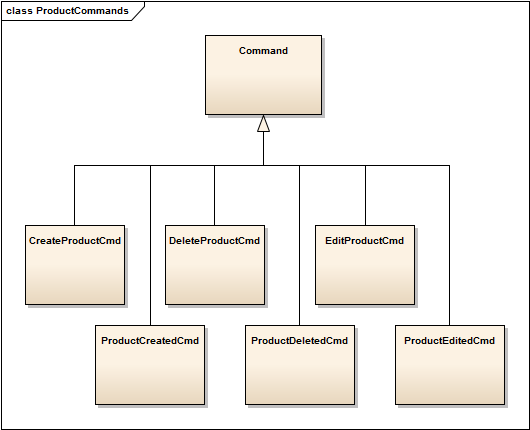
\includegraphics[width=0.6\textwidth]{Systemdesign/SharedLib/Images/Commands/ProductCommands.png}
    \caption{Oversigt over produktspecifikke kommandoer der nedarver fra Command klassen}
    \label{fig:overklassePrd}
\end{figure}

\textbf{Produktkategori kommadoer} er kommando klasser der er specifikke for ProductCategory klassen og disse medfører ændringer i den produktkategori der refereres. Et eksempel herpå kunne være DeleteProductCategoryCmd, der beder \gls{CS} om at slette den givne produktkategori fra databasen.

På figur \ref{fig:overklassePrdCat} ses en oversigt over de forskellige produktkategori kommandoer der nedarver fra Command klassen.

\begin{figure}[H]
    \centering
    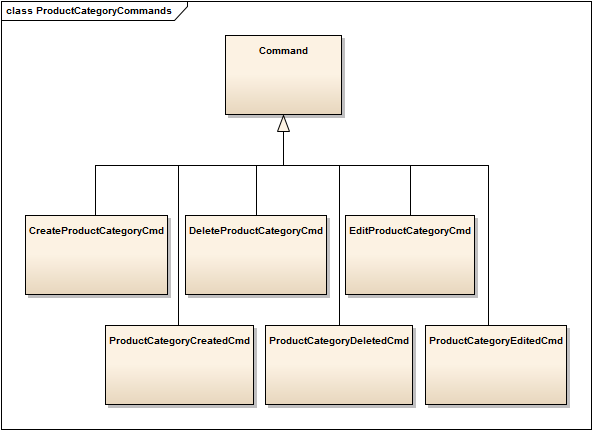
\includegraphics[width=0.6\textwidth]{Systemdesign/SharedLib/Images/Commands/ProductCategoryCommands.png}
    \caption{Oversigt over produktkategori-specifikke kommandoer der nedarver fra Command klassen}
    \label{fig:overklassePrdCat}
\end{figure}



\subsubsection{Klassebeskrivelser}
Herunder forklares yderligere om de forskellige kommando klasser der findes i \gls{SL}. Der vil desuden være en uddybende forklaring om de forskellige klassers funktionalitet og ansvar.\\

\textbf{Command}\\
Denne klasse indeholder blot en attribut, nemlig CmdName. Alle andre kommandoer i \gls{SL} nedarver fra denne klasse hvilket betyder at det bliver muligt at kode op imod en Command klasse og ved at caste på baggrund af CmdName, kan man generisk lave funktionalitet på modtagne kommando objekter, hvilket blandt andet bliver udnyttet i de forskellige marshallers Decode funktion.

\begin{figure}[H]
    \centering
    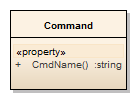
\includegraphics[width=0.2\textwidth]{Systemdesign/SharedLib/Images/Klasser/Command/Command.png}
    \caption{Command}
    \label{fig:klasseCMDCommand}
\end{figure}

\subsubsection*{Generelle kommandoer}

\textbf{RegisterPurchaseCmd}\\
Denne klasse indeholder en liste af købte produkter, PurchasedProduct objekter, og har til hensigt at sende en Purchase instans til \gls{CS} der her sørger for at gemme denne i databasen. Alt dette giver muligheden for at gemme tidligere salg, til senere evt. at kunne lave statistikker (fremtidigt arbejde) eller generere salgskviterringer og rekvisitionskvitteringer.

\begin{figure}[H]
    \centering
    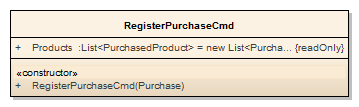
\includegraphics[width=0.6\textwidth]{Systemdesign/SharedLib/Images/Klasser/Command/RegisterPurchase.png}
    \caption{RegisterPurchaseCmd}
    \label{fig:klasseCMDRegP}
\end{figure}

\textbf{GetCatalogueCmd}\\
Denne klasse har intet indhold og dækker i virkeligheden kun et overfladisk behov for at kunne anmode om at få produktkataloget fra \gls{CS}. Derfor er Command klassens nedarvede attribut CmdName det eneste der er behov for i denne klasse.

\begin{figure}[H]
    \centering
    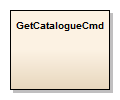
\includegraphics[width=0.2\textwidth]{Systemdesign/SharedLib/Images/Klasser/Command/GetCatalogue.png}
    \caption{GetCatalogueCmd}
    \label{fig:klasseCMDGetC}
\end{figure}

\textbf{CatalogueDetailsCmd}\\
Denne klasse er et modsvar til kommandoen GetCatalogue der anmoder om produktkataloget fra \gls{CS}, og vil derfor blive sendt som et modsvar med en liste af produktkategorier.

\begin{figure}[H]
    \centering
    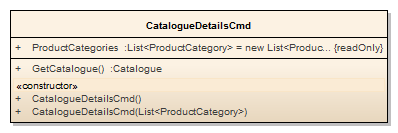
\includegraphics[width=0.6\textwidth]{Systemdesign/SharedLib/Images/Klasser/Command/CatalogueDetails.png}
    \caption{CatalogueDetailsCmd}
    \label{fig:klasseCMDGetC}
\end{figure}

\subsubsection*{Produkt kommandoer}

\textbf{CreateProductCmd/ProductCreatedCmd}\\
Disse klasser er skabt for henholdsvis at oprette et produkt i databasen og derefter en kommando der bliver sendt ud med information om at et nyt produkt er blevet oprettet. CreateProduct klassen indeholder alle de samme attributter som Product klassen med undtagelse af et produkt id da dette først er noget \gls{CS} tildeler produktet når det bliver oprettet i databasen. Derfor er der naturligvis en ekstra attribut i ProductCreated, der hedder ProductId, som er dette id der er blevet tildelt produktet, og som senere kan bruges som reference til dette produkt.

\begin{figure}[H]
    \centering
    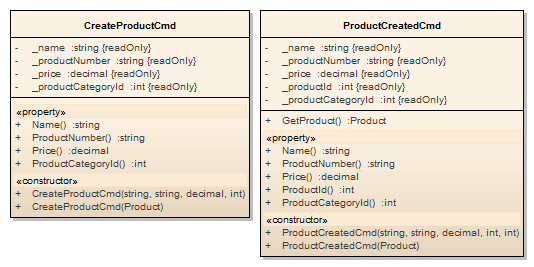
\includegraphics[width=0.8\textwidth]{Systemdesign/SharedLib/Images/Klasser/Command/Product/CreatePrd.png}
    \caption{CreateProductCmd/ProductCreatedCmd}
    \label{fig:klasseCMDCreatePrd}
\end{figure}

\textbf{DeleteProductCmd/ProductDeletedCmd}\\
DeleteProduct og ProductDeleted er to klasser med praktisk talt samme informationer. Den springende forskel er blot at DeleteProduct bliver sendt til \gls{CS} for at bede denne om at slette produktet fra databasen, og ProductDeleted er et svar fra \gls{CS} ud til alle interessanter om at det omtalte produkt er blevet slettet fra databasen.
Klasserne indeholder naturligvis samme attributter som Product klassen da disse informationer kan være relevante for de forskellige modtagere. For at anmode om sletning af et produkt kan man dog blot nøjes med at sende produkt id'et med kommandoen og ud fra dette kan \gls{CS} finde produktet i databasen og slette det.

\begin{figure}[H]
    \centering
    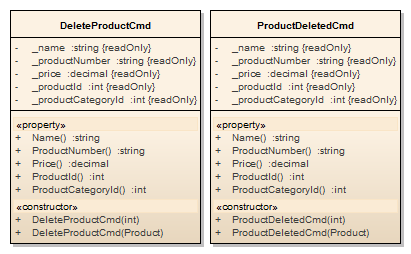
\includegraphics[width=0.6\textwidth]{Systemdesign/SharedLib/Images/Klasser/Command/Product/DeletePrd.png}
    \caption{DeleteProductCmd/ProductDeletedCmd}
    \label{fig:klasseCMDDeletePrd}
\end{figure}

\textbf{EditProductCmd/ProductEditedCmd}\\
Disse klasser bruges af de forskellige systemer til at lave ændringer i et allerede eksisterende produkt, f.eks. hvis et produkts name attribute er stavet forkert, så kan der sendes et EditProduct objekt med de reviderede informationer til \gls{CS} og denne vil herefter sørge for at rette disse informationer i databasen. ProductEdited kommandoen er herefter de opdaterede informationer der bliver sendt ud til alle interessanter i systemet. De to klasser indeholder derfor også alle de samme informationer som Product klassen og der kan på den måde også ændres flere informationer på et produkt i samme kommando.

\begin{figure}[H]
    \centering
    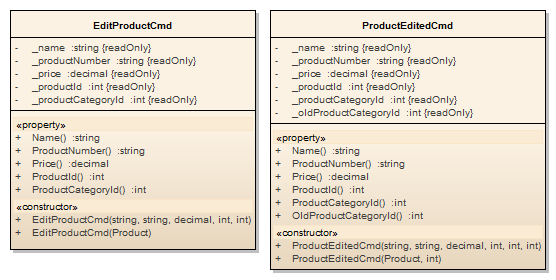
\includegraphics[width=0.8\textwidth]{Systemdesign/SharedLib/Images/Klasser/Command/Product/EditPrd.png}
    \caption{EditProductCmd/ProductEditedCmd}
    \label{fig:klasseCMDDeletePrd}
\end{figure}

\subsubsection*{Produktkategori kommandoer}

\textbf{CreateProductCategoryCmd/ProductCategoryCreatedCmd}\\
Disse klasser er skabt for at oprette en produktkategori i databasen, CreateProductCategory anmoder \gls{CS} om dette og derefter sender denne en ProductCategoryCreated kommando ud med information om at en ny produktkategori er blevet oprettet. CreateProductCategory klassen indeholder alle de samme attributter som ProductCategory klassen med undtagelse af et produktkategori id da dette først er noget \gls{CS} tildeler produktkategorien når denne bliver oprettet i databasen. Derfor er der naturligvis en ekstra attribut i ProductCategoryCreated, der hedder ProductCategoryId, som er det id der er blevet tildelt produktkategorien, og som senere kan bruges som reference til denne produktkategori. 

\begin{figure}[H]
    \centering
    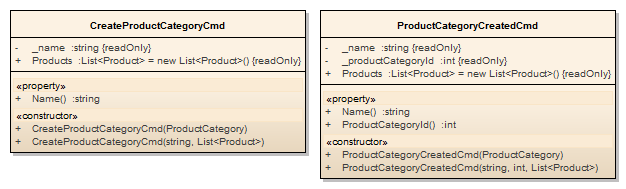
\includegraphics[width=1.0\textwidth]{Systemdesign/SharedLib/Images/Klasser/Command/ProductCategory/CreatePrdCtg.png}
    \caption{CreateProductCategoryCmd/ProductCategoryCreatedCmd}
    \label{fig:klasseCMDCreatePrdCtg}
\end{figure}

\textbf{DeleteProductCategoryCmd/ProductCategoryDeletedCmd}\\
DeleteProductCategory og ProductCategoryDeleted er to klasser med praktisk talt samme informationer. Den springende forskel er blot at DeleteProductCategory bliver sendt til \gls{CS} for at bede denne om at slette produkkategorien fra databasen, og ProductCategoryDeleted er et svar fra \gls{CS} ud til alle interessanter om at den omtalte produktkategori er blevet slettet fra databasen.
Klasserne indeholder naturligvis samme attributter som ProductCategory klassen da disse informationer kan være relevante for de forskellige modtagere. For at anmode om sletning af en produktkategori kan man dog blot nøjes med at sende produktkategori id'et med kommandoen og ud fra dette kan \gls{CS} finde produktkategorien i databasen og slette den.


\begin{figure}[H]
    \centering
    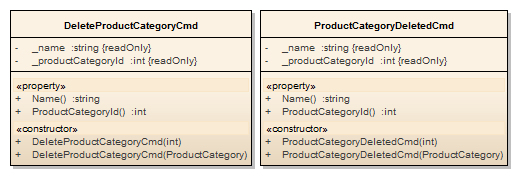
\includegraphics[width=0.8\textwidth]{Systemdesign/SharedLib/Images/Klasser/Command/ProductCategory/DeletePrdCtg.png}
    \caption{DeleteProductCategoryCmd/ProductCategoryDeletedCmd}
    \label{fig:klasseCMDDeletePrdCtg}
\end{figure}

\textbf{EditProductCategoryCmd/ProductCategoryEditedCmd}\\
Disse klasser bruges af de forskellige systemer til at lave ændringer i et allerede eksisterende produktkategorier, f.eks. hvis en produktkateogri's name attribute er stavet forkert, så kan der sendes et EditProductCategory objekt med de reviderede informationer til \gls{CS} og denne vil herefter sørge for at rette disse informationer i databasen. ProductCategoryEdited kommandoen er herefter de opdaterede informationer der bliver sendt ud til alle interessanter i systemet. De to klasser indeholder derfor også alle de samme informationer som ProductCategory klassen og der kan på den måde også ændres flere informationer på et produktkategori i samme kommando.


\begin{figure}[H]
    \centering
    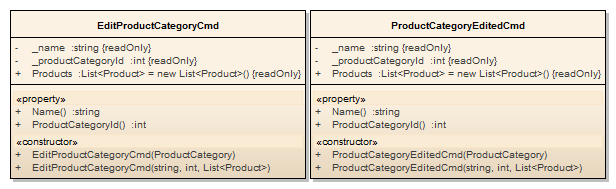
\includegraphics[width=1.0\textwidth]{Systemdesign/SharedLib/Images/Klasser/Command/ProductCategory/EditPrdCtg.png}
    \caption{EditProductCategoryCmd/ProductCategoryEditedCmd}
    \label{fig:klasseCMDEditPrdCtg}
\end{figure}




\subsection{XmlMarshaller}
XmlMarshalleren er en klasse der implementerer IProtocolMarshal interfacet, Der vil i fremtiden være flere af disse protokol marshallers så den sendte kode kunne være andet end XML, men da det var fokuspunktet for dette projekt er der kun skabt denne ene. Dog med et interface så der stadig er mulighed for at udbygge systemet. XmlMarshalleren har til ansvar at fjerne postfix navnet "Cmd" fra det objekt der er kaldt enten encode eller decode på, Og vil så herefter søge i \gls{SL}'s mappestruktur efter en lignende klasse blot med postfix "Marshal", hvis denne findes vil der blive kaldt den givne kommando, (enten encode eller decode) på denne marshaller. Hvis ikke marshalleren findes vil der tilgengæld blive smidt en exception med en meddelelse om at marshalleren ikke findes. 

\begin{figure}[H]
	\centering
	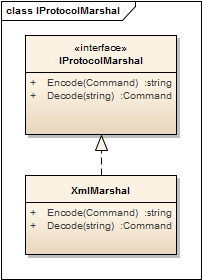
\includegraphics[width=0.4\textwidth]{Systemdesign/SharedLib/Images/Klasser/IProtocolMarshal.png}
	\caption{XmlMarshal der implementerer IProtocolMarshal}
	\label{fig:klasseXmlMar}
\end{figure}

\subsection{Marshallers} \label{MARSHALLER}

Protokollens hovedfunktionalitet ligger i det der her i systemet kaldes "Marshallers", Hver enkelt kommando klasse har en tilsvarende marshaller der er skræddersyet til at håndtere de attributter der er specifikke for netop den klasse. Derfor skelnes der på samme måde som kommandoer imellem tre typer af marshallers:

\begin{itemize}
	\item \textbf{Generelle marshallers} 
	\item \textbf{Produkt marshallers} 
	\item \textbf{Produktkategori marshallers}
\end{itemize}

Alle tre typer af marshallers implementerer interfacet ICmdMarshaller, og indeholder derfor kun to funktioner.

\begin{itemize}
	\item \textbf{Encode()} 
	\item \textbf{Decode()} 
\end{itemize}

Selve implementeringen af disse funktioner er dog så forskellig at det har været nødvendigt at lave marshallers for hver kommando. Denne design beslutning gav dog også systemet den fordel at det designmæssigt er klart til eventuelle udvidelser uden at skulle ændre i eksisterende funktionalitet og dermed overholder Open-Closed princippet.

\subsubsection{Klassebeskrivelser}
Da UML'en i de forskellige marshallers praktisk talt ligner hinanden er diagrammerne i denne klassebeskrivelse slået sammen til oversigter over de tre typer af marshallers hvortil der vil være en kort beskrivelse af de enkelte klasser.\\

\textbf{Generelle marshallers} håndterer de generelle kommandoer. på figur \ref{fig:overklasseMarsGen} ses en oversigt over de forskellige generelle marshal klasser der alle implementerer ICmdMarshal interfacet.

\begin{figure}[H]
	\centering
	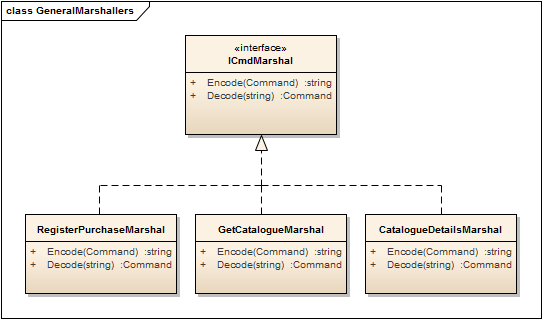
\includegraphics[width=0.8\textwidth]{Systemdesign/SharedLib/Images/Marshallers/GeneralMarshallers2.png}
	\caption{Oversigt over generelle marshallers der nedarver fra ICmdMarshal klassen}
	\label{fig:overklasseMarsGen}
\end{figure}

På figur \ref{fig:overklasseMarsGen} ses først \textit{RegisterPurchaseMarshal}, denne håndterer selvfølgelig RegisterPurchase kommandoen. Dennes encode/decode funktion skal derfor kunne tage højde for et Purchase objekt med en liste af PurchasedProducts og få disse omsat i korrekt format og ligeledes tilbage til de korrekte objekter. 

GetCatalogue kommandoen har i sig selv ingen logik, for yderligere information se figur \ref{fig:klasseCMDGetC}, men dette betyder dog stadig at \textit{GetCatalogueMarshal} skal parse kommando navnet, da det er dette \gls{CS} handler på baggrund af. 

\textit{CatalogueDetailsMarshal} håndterer CatalogueDetails kommandoen og skal derfor kunne parse en liste af ProductCategory objekter der hver især indeholder en liste af Product objekter. Dette gav i første omgang en del problemer da systemet fik indført produktkategorier da det praktisk talt krævede en total revidering af denne klasse.\\


\textbf{Produkt marshallers} håndterer alle de produkt specifikke kommandoer. på figur \ref{fig:overklasseMarsP} ses en oversigt over de forskellige produkt marshal klasser der alle implementerer ICmdMarshal interfacet.

\begin{figure}[H]
	\centering
	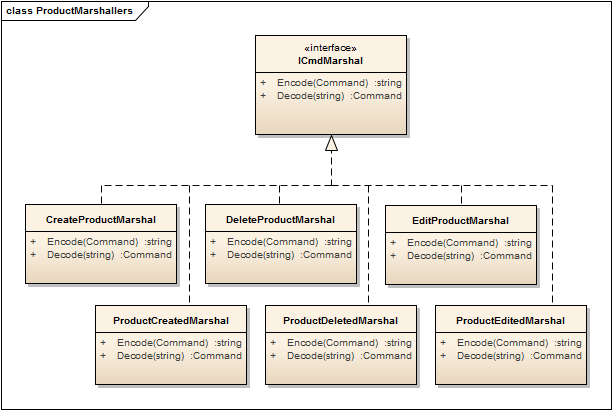
\includegraphics[width=0.8\textwidth]{Systemdesign/SharedLib/Images/Marshallers/ProductMarshallers2.png}
	\caption{Oversigt over produkt specifikke marshallers der implementerer ICmdMarshal interfacet}
	\label{fig:overklasseMarsP}
\end{figure}

På figur \ref{fig:overklasseMarsP} ser den oplyste læser hurtigt at produkt marshallerne på samme måde som kommandoerne kan sættes i par. \textit{CreateProductMarshal} og \textit{ProductCreatedMarshal} håndterer henholdsvis CreateProduct og ProductCreated kommandoerne og skal derfor sørge for at parse Product attributter til og fra XML.

Derefter kommer \textit{DeleteProductMarshal} og \textit{ProductDeletedMarshal} der håndterer henholdsvis DeleteProduct og ProductDeleted kommandoerne, disse skal ligeledes sørge for at parse simple attributter.

Sidst kommer \textit{EditProductMarshal} og \textit{ProductEditedMarshal} der håndterer henholdsvis EditProduct og ProductEdited kommandoerne, disse skal på samme måde som de tidligere marshallers af samme type parse produkt specifikke attributter til og fra XML.\\



\textbf{Produktkategori marshallers} håndterer alle de produktkategori specifikke kommandoer. på figur \ref{fig:overklasseMarsPC} ses en oversigt over de forskellige produktkategori marshal klasser der alle implementerer ICmdMarshal interfacet.

\begin{figure}[H]
	\centering
	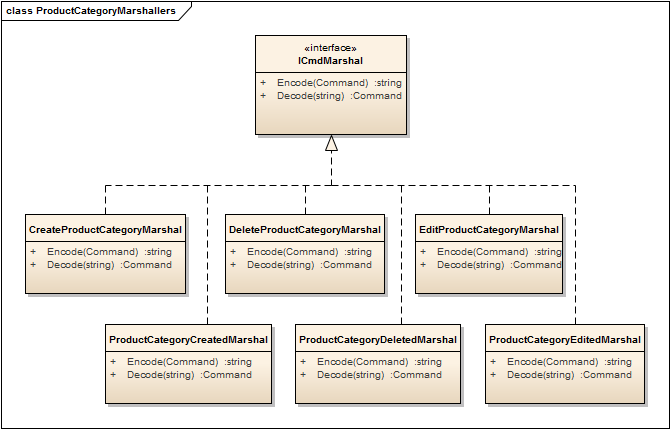
\includegraphics[width=0.8\textwidth]{Systemdesign/SharedLib/Images/Marshallers/ProductCategoryMarshallers2.png}
	\caption{Oversigt over produktkategori specifikke marshallers der nedarver fra ICmdMarshal klassen}
	\label{fig:overklasseMarsPC}
\end{figure}

På figur \ref{fig:overklasseMarsP} ses det meget lignende produkt marshallerne at produktkategori marshallerne på samme måde som kommandoerne kan sættes i par. \textit{CreateProductCategoryMarshal} og \textit{ProductCategoryCreatedMarshal} håndterer henholdsvis CreateProductCategory og ProductCategoryCreated kommandoerne og skal derfor sørge for at parse et ProductCategory objekt med en liste af Product objekter og deres attributter til og fra XML.

Derefter kommer \textit{DeleteProductCategoryMarshal} og \textit{ProductCategoryDeletedMarshal} der håndterer henholdsvis DeleteProductCategory og ProductCategoryDeleted kommandoerne, disse skal ligeledes sørge for at parse et ProductCategory objekt med en liste af Product objekter og deres attributter.

Sidst kommer \textit{EditProductCategoryMarshal} og \textit{ProductCategoryEditedMarshal} der håndterer henholdsvis EditProductCategory og ProductCategoryEdited kommandoerne, disse skal på samme måde som de tidligere marshallers af samme type parse et ProductCategory objekt med en liste af Product objekter og deres attributter til og fra XML.\\




\subsection{Threading}
For at simplificere opstart af tråde er klassen ThreadStarter blevet implementeret. Dens statiske metode, Start() tager imod objekter, som implementerer interfacet IThreadRunner. Disse objekter får kald RunThread(), hvori tråden eksekveres. ThreadStarter.Start() returnerer et .NET Thread objekt, som allerede er startet. Gennem Thread objektet kan tråden manipuleres (Stop, Join mv.).

\begin{figure}[H]
    \centering
    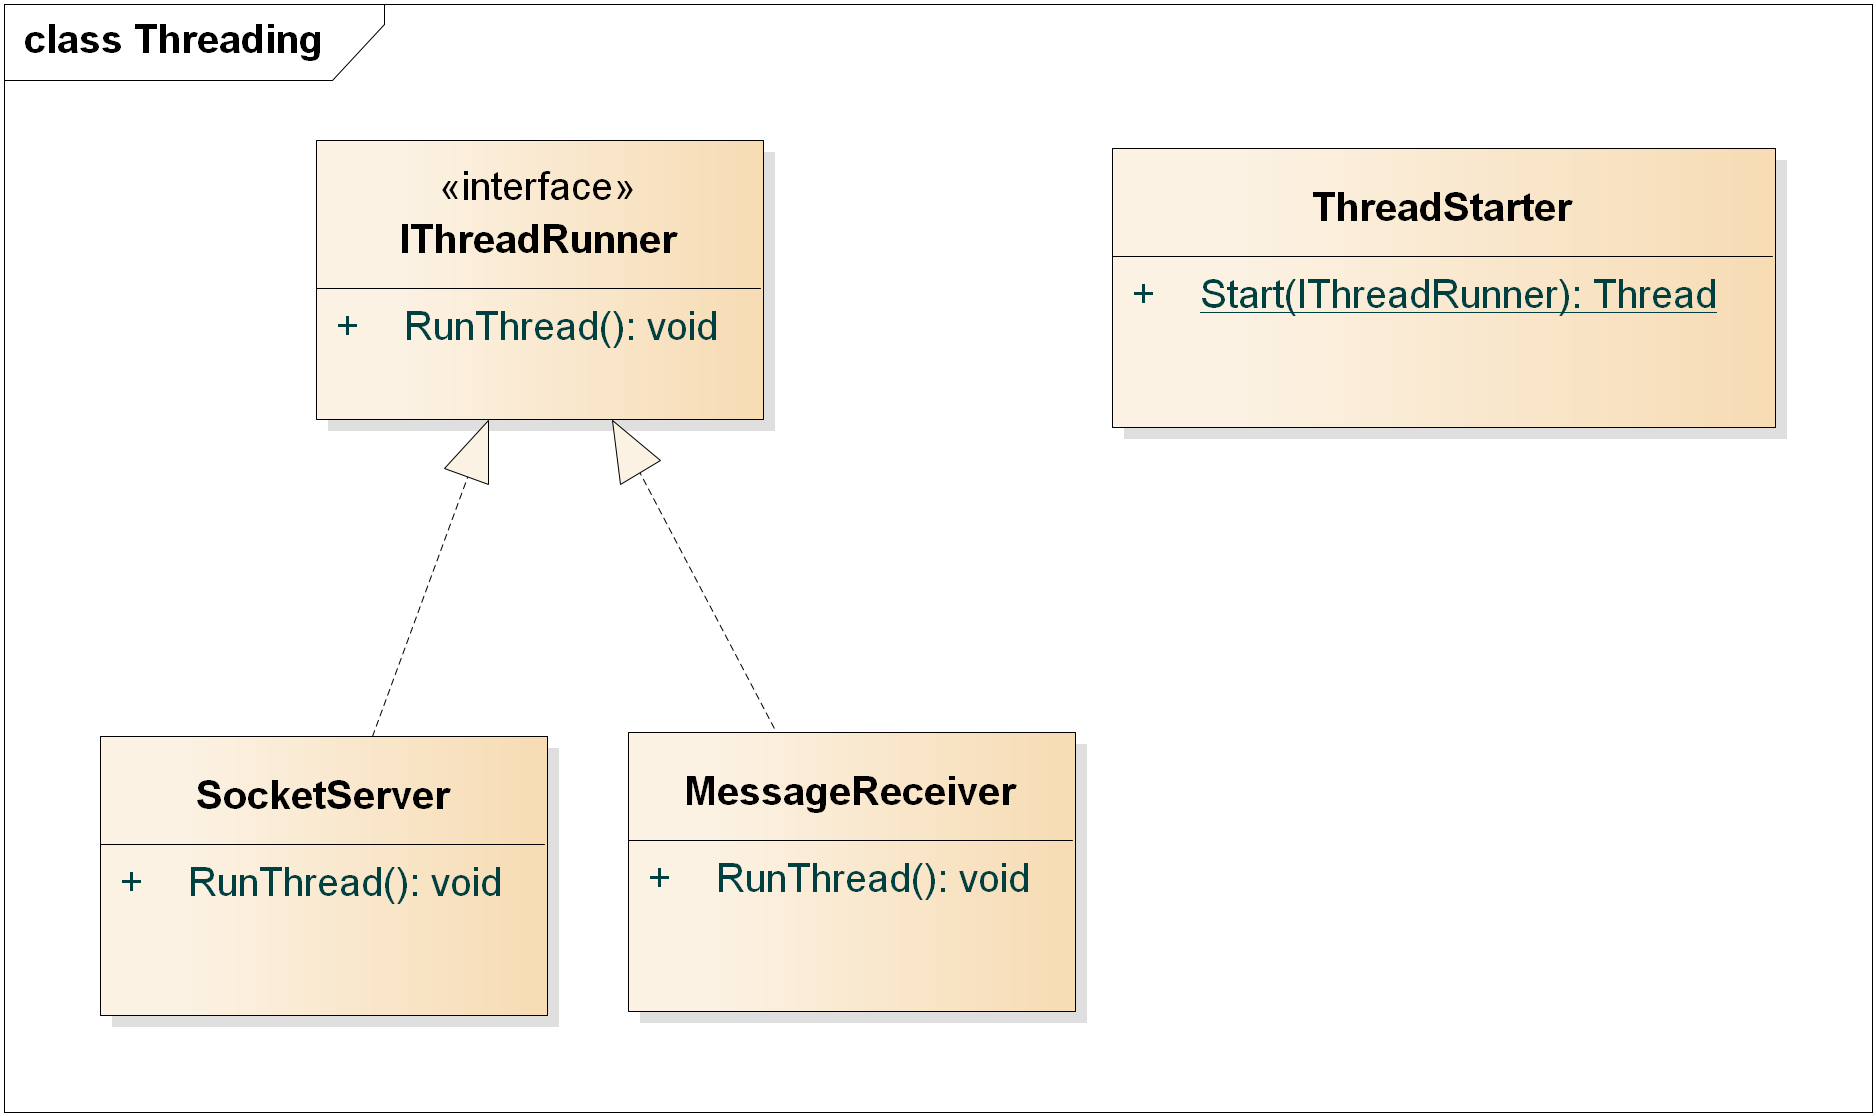
\includegraphics[width=1\textwidth]{Systemdesign/CentralServer/Images/Threading.png}
    \caption{UML-diagram for Threading pakken}
    \label{fig:CSThreading}
\end{figure}

I CentralServer implementerer følgende klasser IThreadRunner interfacet: SocketServer og MessageReceiver.
\textbf{Klient}
Sockets består af hhv. en klient til at sende, og en klasse der kan lytte. Klienten som sender fungerer asynkront, således at der ikke blokeres i en eventuel GUI, hvis det er her denne bruges. Det ses at dette bruges eksempelvis i \gls{AS}, hvor denne bruges til at sende data til \gls{CS}.\\
Der findes desuden nogle events i denne. Disse indebærer bl.a. 	et event når data er modtaget, og et event hvis der sker en fejl. Dette tillader at der kan implementeres egne handlere, parsere mv. Dette kunne eksempelvis være dem der også findes i \gls{SL} \\\\
 

\textbf{Listener}
Denne klasse implementerer eventhandlere, som reagerer når eventet for data modtaget bliver raised. Denne kontrollerer da hvilken type command\footnote{Commands er nærmere beskrevet i afsnit \ref{COMMANDS} side \pageref{COMMANDS}} der er modtaget. Efterfølgende bliver der således raised et nyt event, som en bruger kan subscribe på, og have sin egen handler.\\
Der findes events for de følgende begivenheder:

\begin{itemize}
	\item Command modtaget
	\item Nyt produkt lavet
	\item Nyt produktkatalog
	\item Ny produktkategori lavet
	\item Produkt er slettet
	\item Produktkategori er slettet
	\item Produktkategori er modificeret
	\item Produkt er modificeret.
\end{itemize}

Selve kommandoen bliver da sendt med, således brugeren selv kan parse denne.\\
På denne måde opnåes en lav kobling. \gls{SL}s klient og listener er komplet uafhængige af hvem der har subscribet på disse events, den raiser dem bare. Ligeledes er der ingen begrænsninger for hvor mange der kan subscribe på disse events. Det tillader da at flere administrationssystemer kan eksistere, og derved blive notificeret hvis der er sket en ændring. Derved opnåes total synkronisering mellem alle subscribere.

\begin{figure}[H]
	\centering
	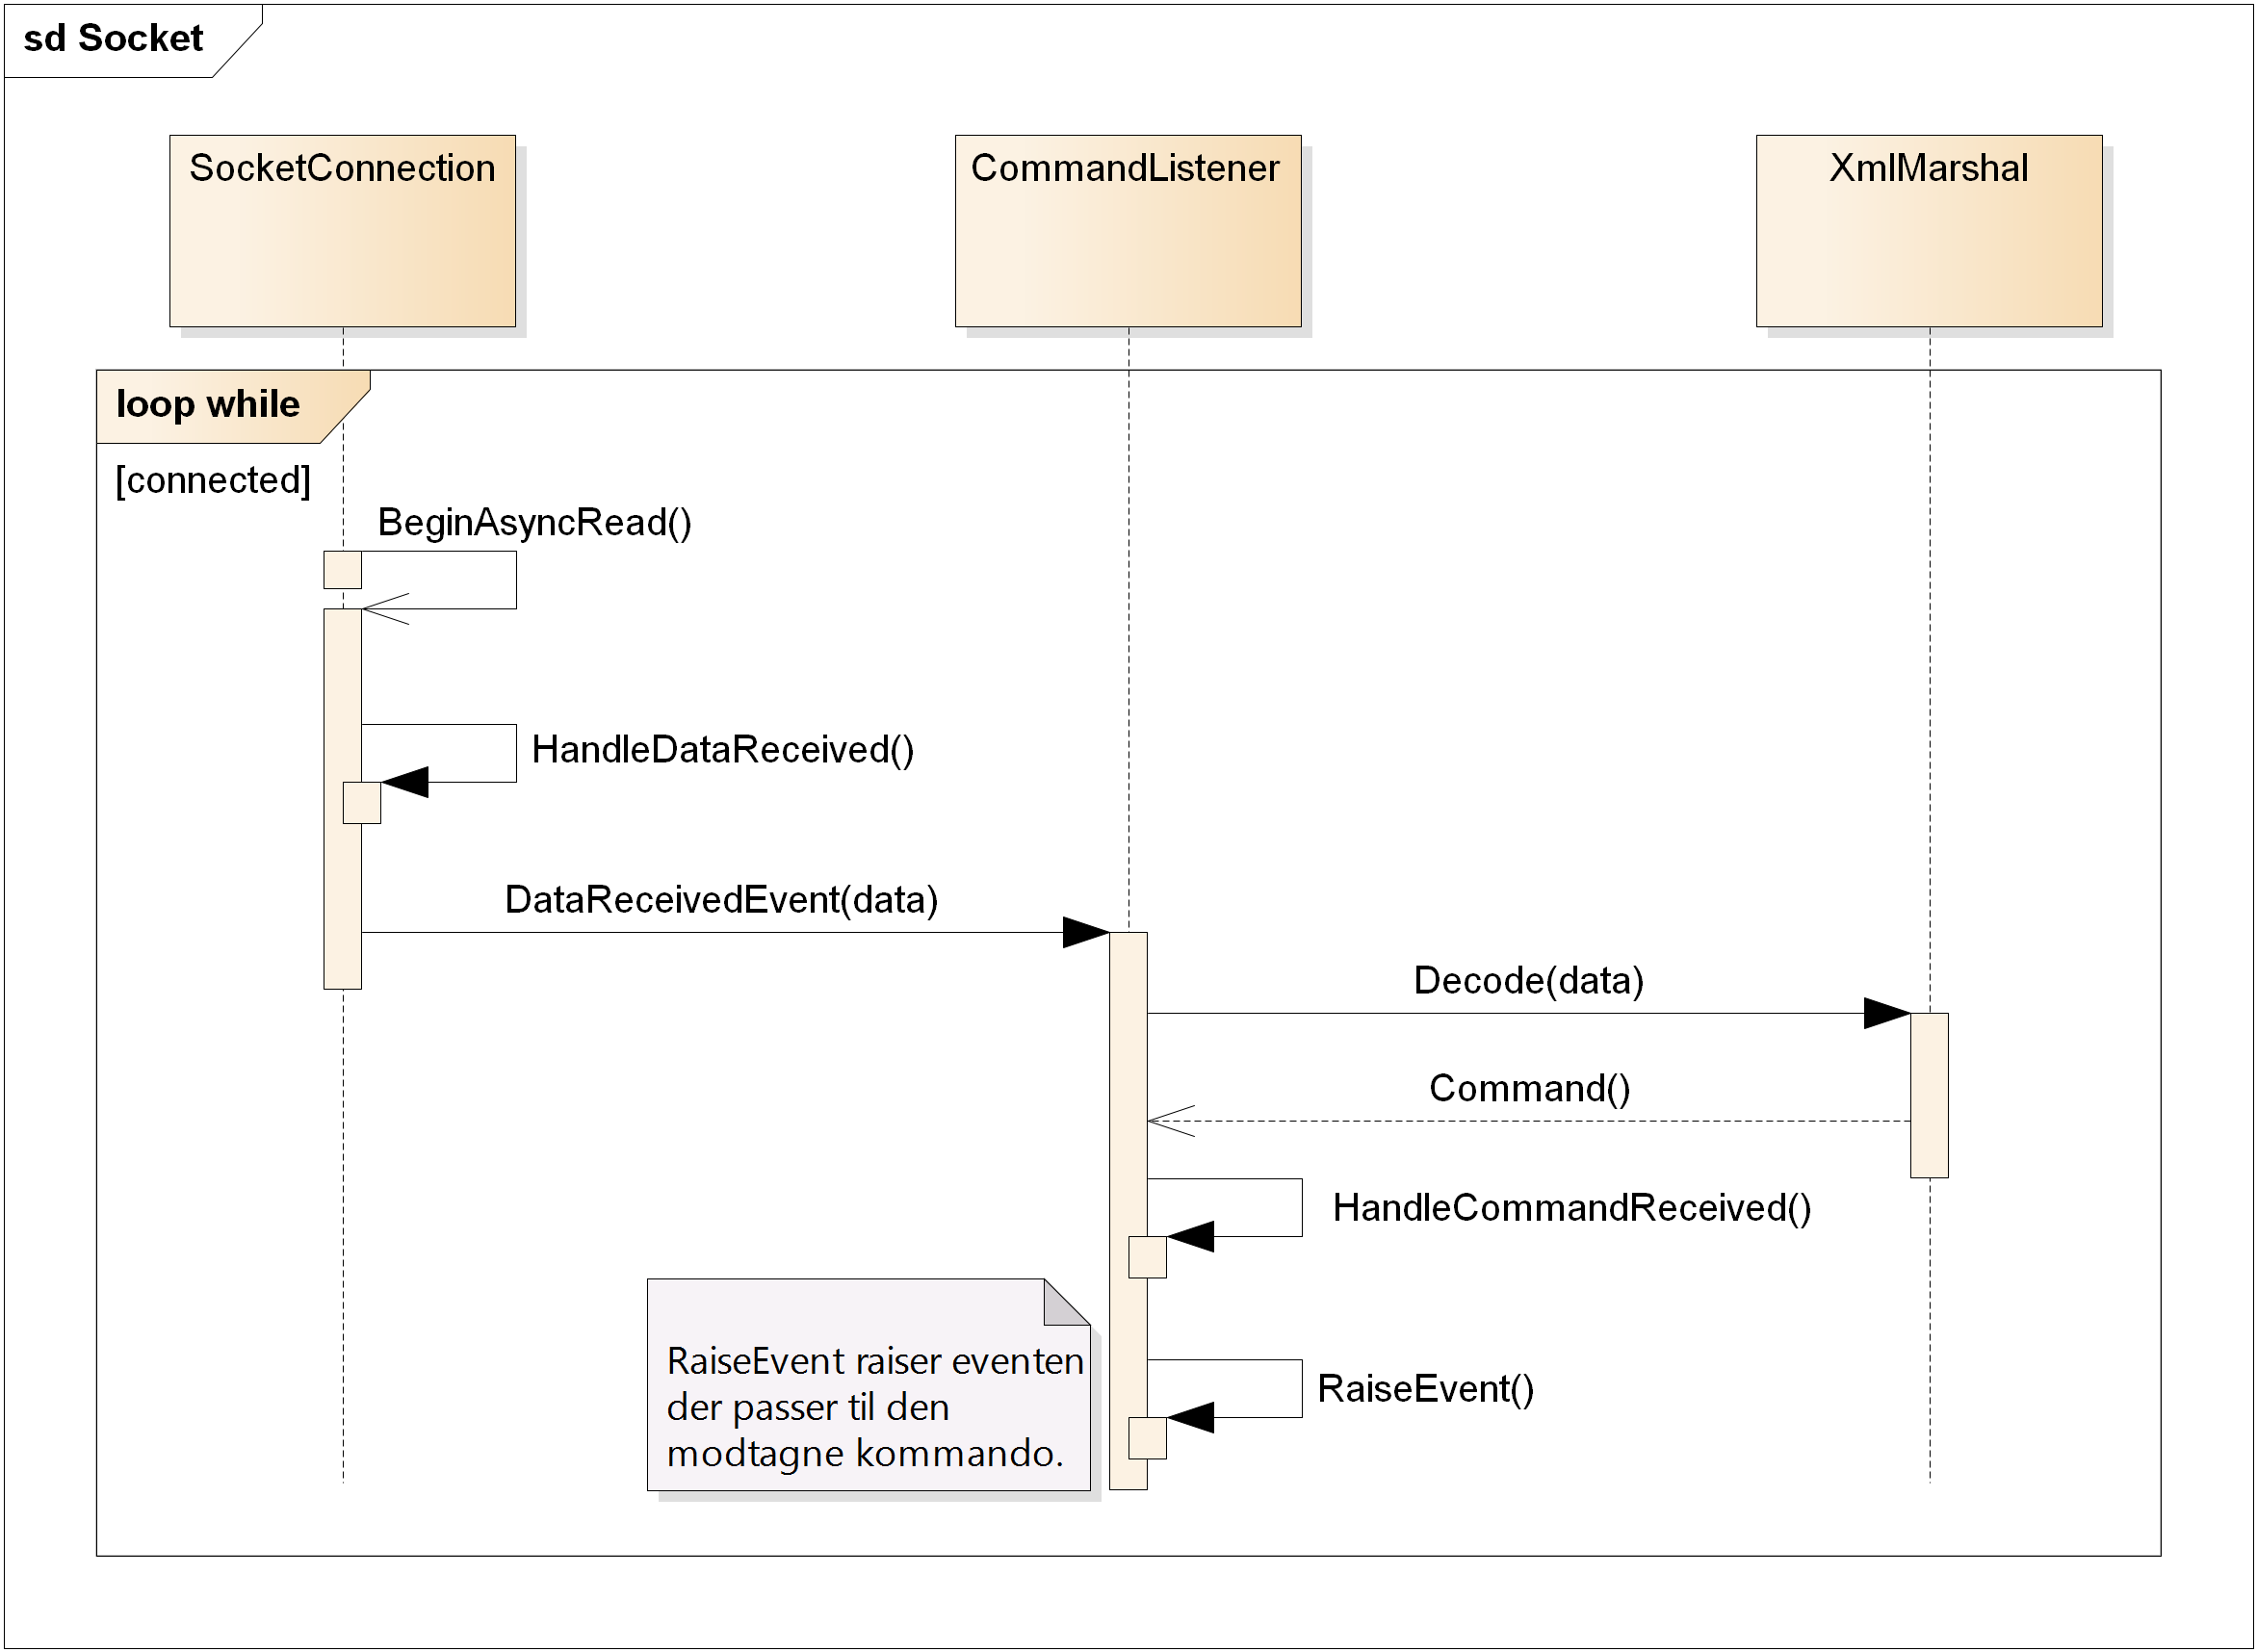
\includegraphics[width=1\textwidth]{Systemdesign/SharedLib/Images/Socket.png}
	\caption{Sekvensdiagram for socketforbindelsen}
	\label{fig:sockit}
\end{figure}

På diagrammet i figur \ref{fig:sockit} ses det hvordan data håndteres. Når den modtages fra serveren. Ved SocketConnection vil read blive ved med at blive kaldt, medmindre der sker en fejl. I dette tilfælde vil et event om fejl blive raised. Se desuden hvordan dataen bearbejdes af modtageren i afsnit \ref{fig:DataReceive} side \pageref{fig:DataReceive}.
 